

\documentclass[12pt]{article}
\usepackage[utf8]{inputenc}
\usepackage{geometry}
\usepackage{svg}
\usepackage{float}
\usepackage{caption}
\usepackage{amsmath,amsthm,amsfonts,amssymb,amscd}
\usepackage{fancyhdr}
\usepackage{titlesec}
\usepackage{xparse}
\usepackage{tikz}
\usetikzlibrary{shapes.geometric, arrows}
\pagestyle{empty}
\titleformat*{\section}{\large\bfseries}

%
\geometry{
 a4paper,
 total={170mm,240mm},
 left=20mm,
 top=30mm,
 }

\date{}
%Bitte ausfüllen
\newcommand\course{Programmierung, Gruppe 16}
\newcommand\hwnumber{1}
\newcommand\Name{Maximilian Petri, 405602}
\newcommand\Neptun{Danje Petersen, 379748}

%Matheinheiten
\newcommand\m{\:\textrm{m}}
\newcommand\M{\:\Big[\textrm{m}\Big]}
\newcommand\mm{\:\textrm{mm}}
\newcommand\MM{\:\Big[\textrm{mm}\Big]}
\newcommand\un{\underline}
\newcommand\s{\:\textrm{s}}
\newcommand\bS{\:\Big[\textrm{S}\Big]}
\newcommand\ms{\:\frac{\textrm{m}}{\textrm{s}}}
\newcommand\MS{\:\Big[\frac{\textrm{m}}{\textrm{s}}\Big]}
\newcommand\mss{\:\frac{\textrm{m}}{\textrm{s}^2}}
\newcommand\MSS{\:\Big[\frac{\textrm{m}}{\textrm{s}^2}\Big]}

%Bitte nicht einstellen

\renewcommand{\thesection}{Aufgabe }
\renewcommand{\thesubsection}{\alph{subsection})}
\renewcommand{\thesubsubsection}{\hspace{0.8cm}\roman{subsubsection})}
\renewcommand{\figurename}{Abbildung}
\renewcommand{\tablename}{Tabelle}
\pagestyle{fancyplain}
\headheight 35pt
\lhead{\Name\\\Neptun}
\chead{\textbf{\Large Hausaufgabe \hwnumber}}
\rhead{\course \\ \today}
\lfoot{}
\cfoot{}
\rfoot{\small\thepage}
\headsep 1.5em

\begin{document}

\section{2)}
\subsection{}
\subsubsection{}
\begin{center}
    Syntax:\bigbreak
    "$p.\:q\::-\:p$" ist kein syntaktisch korrektes Wort, da es nicht mit einem "." endet.
\end{center}

\subsubsection{}
\begin{center}
    Syntax:
    $$ S_2 \quad \rightarrow \quad A.S_2 \quad \rightarrow \quad B.S_2 \quad \rightarrow \quad p.S_2 $$
    $$\rightarrow \quad p.A.S_2 \quad \rightarrow \quad p.B:-B.S_2 \quad \rightarrow \quad p.q:-p.S_2$$
    $$ \rightarrow \quad p.q:-p.A. \quad \rightarrow \quad p.q:-p.B:-B. \quad \rightarrow \quad p.q:-p.s:-r.$$
    \bigbreak
    Hiermit ist gezeigt das "$p.q:-p.s:-r.$" ein syntaktisch korrektes Wort ist.
    \bigbreak
    Semantik:
    $$ W(p.q:-p.s:-r.) \quad = \quad W(p.q:-p.) \cup \varnothing \quad = \quad W(p.)\cup \varnothing \cup \varnothing \quad = \quad \{ p \} $$
\end{center}

\subsubsection{}
\begin{center}
    Syntax:
    $$ S_2 \quad \rightarrow \quad A. \quad \rightarrow \quad B:-B. $$
    \bigbreak
    Das es kein Terminal "$a$" gibt, kann man ab hier nicht weiter ableiten. Deswegen ist das Wort "$a :- r.$" syntaktisch falsch. 
\end{center}

\subsection{}
\begin{center}
    Zwei Wörter mit gleicher Semantik müssen \underline{nicht} die gleiche Syntax haben. Zum Beispiel die Wörter "Fehrnbedienung" und "Drücker" in der deutschen Sprache meinen im richtigen Kontext beide das Gleiche, aber ihre Syntax ist unterschiedlich.
\end{center}

\subsection{}
\begin{center}
    Damit ein Wort semantisch Korrekt ist, muss es syntaktisch Korrekt sein, weil es sonst nicht zur Sprache gehört.
\end{center}
 \pagebreak %|||||||||||||||||||||||||||||||||||||||||||||||||||
 
 

\section{4)}
\subsection{}
\begin{center}
    G($L_2$) = $(\{S, A, B, X\}, \{a, b\}, P, S)$ \\
\end{center}
\begin{center}
  \begin{tabular}{l}
    P=\{ \\
    \quad$S \rightarrow \quad B \quad|\quad X \quad|\quad \epsilon$ \\
    \quad$B \rightarrow \quad bB \quad|\quad b $ \\
    \quad$X \rightarrow \quad aXb \quad|\quad Xab \quad|\quad abX \quad|\quad A$ \\
    \quad$A \rightarrow \quad aA \quad|\quad a $ \\
    \}
 \end{tabular}
\end{center}

\subsection{}
\begin{center}
 \begin{tabular}{l}

    $ S_1 = \{\quad a,\quad [S_2]\quad\} $ \\
    $ S_2 = [\quad (b \quad|\quad a, \quad S_2)\quad] $
 \end{tabular}
\end{center}

\subsection{}
\begin{figure}[h]
    \centering
    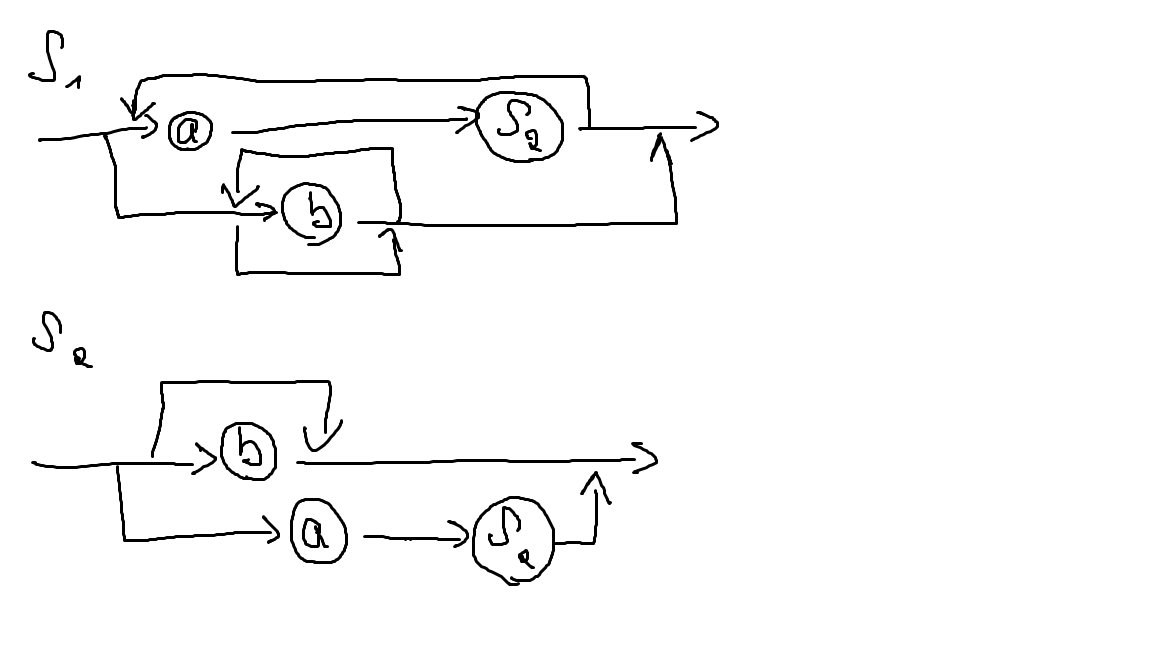
\includegraphics[width = 1\textwidth]{progradiagramm.png}
    \caption{}
    \label{}
\end{figure}

\pagebreak %|||||||||||||||||||||||||||||||||||||||||||||||||||||||

\section{6)}

\subsection{}
\subsubsection{}
$$ (0101010101)_2 = (2^8+2^6+2^4+2^2+2^0)_{10} = (341)_{10} $$
\subsubsection{}
$$ (1000000000)_2 = K_2(1000000000)_2 = K_1(1000000000)_2 + 1 = -(1000000000)_2 = -(1024)_{10} $$
\subsubsection{}
$$ (0100101110)_2 = (2^8 + 2^5 + 2^3+2^2+2^1)_{10} = (302)_{10}$$
\subsubsection{}
$$ (1100011001)_2 = K_2(1100011001)_2 = -(0011100111)_2 = -(231)_{10} $$
\subsubsection{}
$$ (1000101110)_2 = K_2(1000101110)_2 = -(0111010010)_2 = -(466)_{10} $$

\subsection{}
\subsubsection{}
\begin{center}
    Da beim "-" in Java standartmäßig die beiden Ganzzahlen als int interpretiert werden und die kleinstmögliche, mit einem int darstellbare, Zahl $-2^{31} = -2147483648$ ist und $-1000000000 -1100000000 -200000000$ kleiner als $-2^{31}$ ist, entsteht hier ein Unterlauf, welcher zur Folge hat das aus der Subtraktion, welcher ja eigentlich kleiner 0 sein sollte, das Ergebnis $1994967296$ hervorgeht.
    Das ist größer 0 und deshalb ergibt der Ausdruck true.
\end{center}
\subsubsection{}
\begin{center}
    $ -(0-2000000000-147000000-483000-648)_{10} = -(-(2147483648)_{10})$
    $ = -(10...0)_2 = -(K_1(10...0)_2+1) = -(-(01...1)_2 + 1) = -(-(10...0)_2) = (10...0)_2$
    $ = K_1(10...0)_2 + 1 = -((01...1)_2 + 1) = -(10...0)_2 = -(2147483648)_{10} < 0$
    \bigbreak
    Mathematisch macht die Rechnung natürlich keinen direkten Sinn, jedoch aufgrund des beschränkten Speicherplatzes auf einem Rechner kann man die kleinste Zahl im $K_2$ immer negieren und man erhält wieder denselben Wert, weil es beim int, mit seinen 32 Bit, kein positives Äquivalent zur kleinsten Zahl ($-2^{31}$) gibt. Versucht man die kleinste darstellbare Zahl für 32 Bit zu negieren, bekommt man als Ergebnis die umgekehrte Zahl, also $2^{31}$. Diese würde dann jedoch 33 Bit belegen, weshalb es zu einem Überlauf kommt, wobei das erste Bit der 33 Bit Zahl abgeschnitten wird und man wieder bei der kleinsten 32 Bit Zahl landet. Da diese ja kleiner 0 ist, ergibt der Ausdruck true.
\end{center}
\end{document}
